\section{Interpolation}
Undoubtedly, one of the pinnacles of numerical methods is trying to find a function that passes through a fixed set of points, in hopes of understading how the this points are related to each other, all this using what is known as an `Interpolating Function' which is a function that passes through all the points of a given set. Many different functions exists for a given set of points, in this package, we have built some of the various methods for interpolating a function; however, despite the simplicity of the method's implementation, a general analysis has been conducted on a specific method of implementing the function evaluation; this analysis will be presented after a brief description of the methods.

The following algorithm implementations that we have realized will be detailed in this section:
\begin{itemize}
    \item Polinomial Interpolation \algoref{alg:Polinomial Interpolation}
    \item Piecewise Linear Interpolation \algoref{alg:Piecewise Linear Interpolation}
    \item Piecewise Cubic Hermite Interpolation \algoref{alg:Piecewise Cubic Hermite Interpolation}
    \item Piecewise Cubic Interpolatory Splines \algoref{alg:Piecewise cubic Interpolatory Splines}
\end{itemize}

All of the algoritmhs have three main parameters, 
\begin{itemize}
    \item \textbf{X}: The x-coordinates of the points we want to interpolate.
    \item \textbf{Y}: The y-coordinates of the points we want to interpolate.
    \item \textbf{U}: The x-coordinates of the points we want to evaluate. This is what we call the mesh.
\end{itemize}
And all of them return the y-coordinates of the points we want to evaluate.

Some of the above algorithms were based uppon C. Moller's reference~\cite{doi:10.1137/1.9780898717952}.

\subsection{Polynomial Interpolation}
This approach performs a polynomial interpolation of a given collection of points; it is one of the fundamental ways of interpolation and the root in the solutions of many error estimation problems. 

The main goal of this interpolation is to find create a polynomial of degree $n-1$ (being $n$ the number of points) that passes through all the points of the set. The algorithm implemented uses the Lagrange interpolation formula~\cite{mathworldLagrange}.
\subsubsection{Examples}
	\paragraph{Example 1}{
\begin{lstlisting}[language=Python]
from BNumMet.Interpolation import polinomial
x = list(np.arange(1, 7, 1))
y = [16, 18, 21, 17, 15, 12]
u = np.arange(0.8, 6.2, 0.05)
v = polinomial(x, y, u)
# Plotting using Matplotlib
plt.plot(u, v, "b-", label="Interpolated")
plt.plot(x, y, "ro", label="Original Points")
plt.legend()
plt.show()
\end{lstlisting}
\begin{figure}[H]
    \centering
    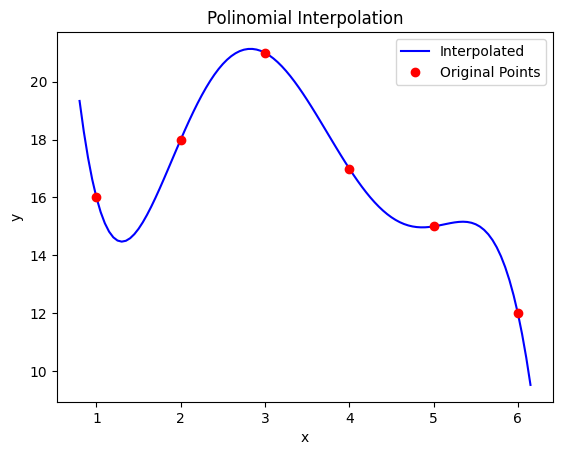
\includegraphics{Include/Images/Thesis/Documentation/Interpolation/Polinomial Example 1.png}
    \caption{Polinomial Linear Example 1}
    \label{fig:Polinomial Linear Example 1}
\end{figure}
}


\subsection{Piecewise linear interpolation}
Following the polynomial interpolation approach, the next step is to extend this notion to piecewise functions; but firstly we will make an intial step using linear functions, that is, we will interpolate the points using a line that passes through two points, this is known as piecewise linear interpolation. 

The way the algorithms works is to find the closest two points from the the point of the mesh all within the given dataset, and the use the calculated slope in order to evaluate the point of the mesh.

\subsubsection{Examples}
	\paragraph{Example 1}{
\begin{lstlisting}[language=Python]
from BNumMet . Interpolation import piecewise_linear
x = list(np.arange(1, 7, 1))
y = [16, 18, 21, 17, 15, 12]
u = np.arange(0.8, 6.2, 0.05)
v = piecewise_linear(x, y, u)
# Plotting using Matplotlib
plt.plot(u, v, "b-", label="Interpolated")
plt.plot(x, y, "ro", label="Original Points")
plt.legend()
plt.show()
\end{lstlisting}
\begin{figure}[H]
    \centering
    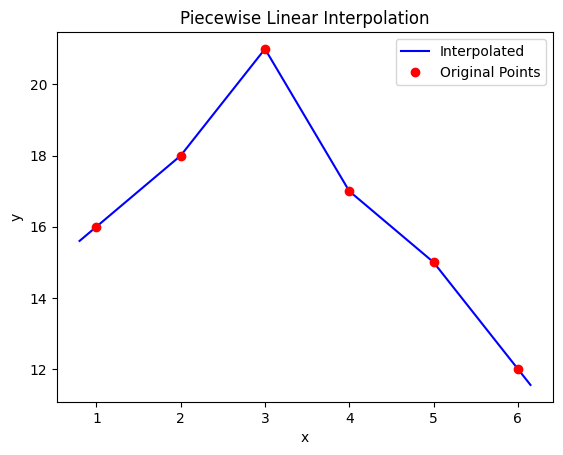
\includegraphics{Include/Images/Thesis/Documentation/Interpolation/PieceWise Linear Example 1.png}
    \caption{PieceWise Linear Example 1}
    \label{fig:PieceWise Linear Example 1}
\end{figure}
}

\subsection{Piecewise cubic interpolation}
Following the Piecewise Linear interpolation we are going to use the same idea but with a cubic function, that is, we will interpolate the points using a cubic function that passes through four points, this is known as piecewise cubic interpolation. 

This interpolating polynomial is twice continuously differentiable, and hence each piecewise function is a cubic spline, as well as, having the boundary conditions know as `not-a-knot'~\cite{doi:10.1137/1.9780898717952} which as Mathwork's states at the first and last interior break, the third derivative of the interpolating function is continuous (up to round-off error)~\cite{notAknot}.


\subsubsection{Examples}
\paragraph{Example 1}{
\begin{lstlisting}[language=Python]
from BNumMet.Interpolation import splines
x = list(np.arange(1, 7, 1))
y = [16, 18, 21, 17, 15, 12]
u = np.arange(0.8, 6.2, 0.05)
v = splines(x, y, u)
# Plotting using Matplotlib
plt.plot(u, v, "b-", label="Interpolated")
plt.plot(x, y, "ro", label="Original Points")
plt.legend()
plt.show()
\end{lstlisting}
\begin{figure}[H]
    \centering
    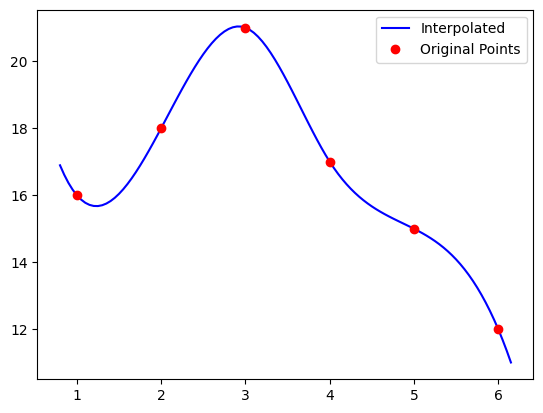
\includegraphics{Include/Images/Thesis/Documentation/Interpolation/Splines Example 1.png}
    \caption{Splines Example 1}
    \label{fig:Splines Example 1}
\end{figure}

}


\subsection{Piecewise Cubic Hermite interpolation}
To end this section, we will present a different approach to piecewise cubic interpolation, this time we will use the Piecewise Cubic Hermite Interpolation Polynomial (P.C.H.I.P.) which is a form of cubic spline interpolation that uses, as per the name indicates, cubic polynomials but whose slopes are explicitly given (in the case of this algorithm they are calcutated according to Mathworks implementation), in the algorithm this is done by looking at the sign of the slopes (using an approximation to the derivative) and then using the harmonic mean to calculate the slope of the interpolating polynomial, this works for the interior points, for the exterior ones . 

The `pchip' function is a Python implementation of the Piecewise Cubic Hermite Interpolation Polynomial (P.C.H.I.P.) based on an old Fortran program by Fritsch and Carlson~\cite{doi:10.1137/0717021}.

\subsubsection{Examples}
	\paragraph{Example 1}{
\begin{lstlisting}[language=Python]
from BNumMet.Interpolation import pchip
x = list(np.arange(1, 7, 1))
y = [16, 18, 21, 17, 15, 12]
u = np.arange(0.8, 6.2, 0.05)
v = pchip(x, y, u)
# Plotting using Matplotlib
plt.plot(u, v, "b-", label="Interpolated")
plt.plot(x, y, "ro", label="Original Points")
plt.legend()
plt.show()
\end{lstlisting}

\begin{figure}[H]
    \centering
    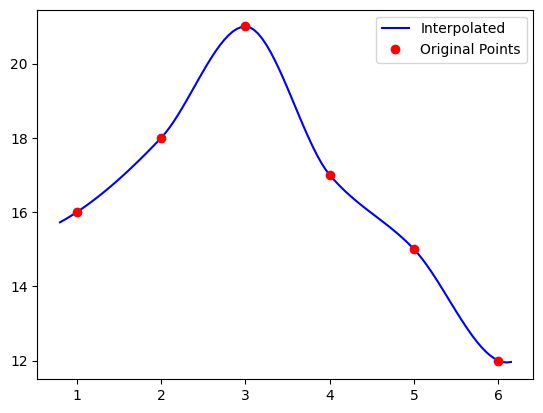
\includegraphics{Include/Images/Thesis/Documentation/Interpolation/PCHIP Example 1.png}
    \caption{PCHIP Example 1}
    \label{fig:PCHIP Example 1}
\end{figure}
}



\subsection{Interpolation implementation analysis}

Similar to the discussion in the linear systems package, we discovered numerous ways a student could implement one part of the method, this one part refers to the lines of code that evaluates the value ($f(x)$) of the points of the mesh. 

In short, for interpolating, one needs to compute the interpolating polynomial as well as evaluating it. The following piece of code is related with the evaluation of piecewise interpolation methods. Particularly, one needs to find in which subinterval a point of the mesh is in, all done to then properly evaluate the interpolating function of that point

The code section may be summarized as follows: 


\begin{algorithm}[H]
\SetAlgoLined
\For{$j \gets 1$ \KwTo $n-2$} {
$k[x_j <= u] \gets j$
}
$s \gets u - x_k$\\
$v \gets y_k + s * \Delta_k$

\caption{Extract from Interpolation's algorithm}
\end{algorithm}
As one can see, this portion of the code assign values to an array $k$ which is then used to access the index of the array $y$ and $x$, this is done in order to apply the specific formula to the approiate section of the mesh. But, we know for a fact that $k$ is an array and we cannot use it as index, per se, thus we need to find a way to access the index of the array $y$ and $x$ using the values of $k$.

Note: It should be noted that other algorithms may have different calculations, however for the sake of simplicity, we are generalizing the portion of code.



We might implement this section of code in a variety of ways, including:
\begin{enumerate}
    \item List Comprehension: Python offers a compact form for adding items to a list, in particular list comprehension, for a general reader a list comprehension is based on mathematical notation that is $\left\{ 3n\ | n\in \mathbb{N},\ 0\leq n\leq 25\right\}$ can be written in Python as \lstinline|[3*n for n in range(0,26)]|, generally speaking list comprehension is faster than classical loops~\cite{PythonSpeedPerformanceTips}, however, a better approach would be using functional maps which are cognitively more difficult to understand, thus not the purpose of this project.
    
    This is an approach that will iterate through the elements in $k$ and therefore we will be able to access the index of the array $y$ and $x$.

    \item Using NumPy's \textit{fancy} Indexing: Similarly to Matlab, NumPy offers a way to broadcast a list, that is we can access the items of a list using another list. This is an approach developed by NumPy that will iterate through the elements in $k$ in a sugar-coated syntax way. In itself, it is a list comprehension but with a different syntax and different internal mechanisms.
    
    Altough it is cognitively more complicated than list comprehensions; it is a syntax that is widely used in the numerical methods realm and might be a fair competitor over list comprehensions.
    
    
    
\end{enumerate}
\paragraph{Results}
To correctly test the implementations we will fix 6 interpolation pairs and then run 100 iterations for different meshes sizes with random values (to also check the ability to sort the mesh points), then after those 100 iterations are over, we will calculate the mean, the results are the following:
\begin{figure}[H]
    \centering
    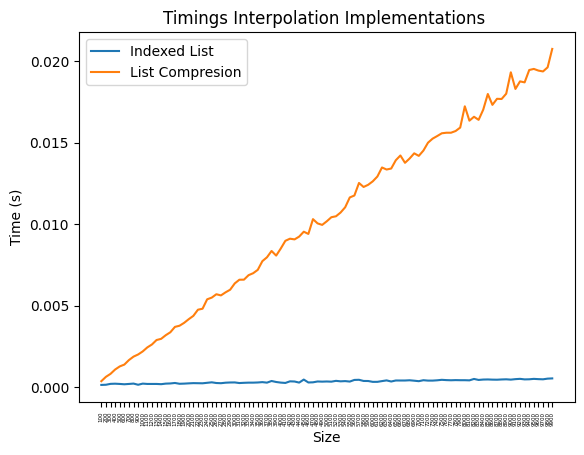
\includegraphics[scale=0.9]{Include/Images/Thesis/Analysis of Solutions/Interpolation/Interpolation Timings.png}
    \caption{Interpolation Timings}
    \label{fig:Interpolation Timings}
\end{figure}

As we can visually observe, the use of List Comprehensions is by far the worst of the two, and should be discarded for this particular case. We can also see how much the \textit{fancy} indexing improves the overall speed.Applying linear regression on both sets of data we get the following results:
\begin{enumerate}
    \item \textbf{Linear Regression \textit{fancy} indexing}: \\
        $y = 3.4812\cdot10^{-08}x + 0.0002$ \\
        Slope: $3.48119\cdot10^{-08}$
    \item \textbf{Linear Regression List Compresion}: \\
        $y = 2.0237\cdot10^{-06}x + 0.0003$ \\
        Slope: $2.02374\cdot10^{-06}$
\end{enumerate}

Overall, not only does the choice of \textit{fancy} indexing is by far the fastest (around 2 orders of magnitude) but it also provides students a syntax that will be used during their learning of numerical methods, though it must be noted, the use of for-loops might be ideal for didactic purposes to teach students what could be behind the notation of this \textit{fancy} indexing.




